\chapter{Metodologia}
Este capítulo objetiva definir a metodologia que será utilizada na pesquisa, bem como apontar quais ferramentas serão usadas na
condução, coleta de dados e análise dos dados.  
\section{Caracterização do Estudo}
A metodologia se refere ao caminho escolhido para se chegar ao fim proposto pela pesquisa. É a escolha que o pesquisador realizou para abordar o objeto de estudo e esta relacionada a relativamente seus elementos essenciais como (natureza, objetivos, procedimentos e abordagens)\cite{de2013metodologia}.

Este tópico tem por objetivo descrever os procedimentos e métodos científicos disponíveis para o desenvolvimento de uma pesquisa, bem como identificar o que melhor se enquadra às necessidades deste trabalho e permitir a reprodução deste trabalho por outros pesquisadores.

\subsection{Do ponto de vista da sua natureza}
No que diz respeito a sua natureza, ou seja, o tipo de contribuição que o estudo trará para a ciência, a pesquisa científica pode ser classificada em: pesquisa básica e pesquisa aplicada.

\textbf{a) pesquisa básica:} objetiva gerar conhecimentos novos úteis para o avanço da ciência sem aplicação prática prevista. Envolve verdades e interesses universais;

\textbf{b) pesquisa aplicada:} objetiva gerar conhecimentos para aplicação prática dirigidos à solução de problemas específicos. Envolve verdades e interesses locais.

\subsection{Do ponto de vista de seus objetivos}

A natureza de uma pesquisa está relacionada com seus objetivos gerais, sendo classicamente rotulada como exploratórias, descritivas ou explicativas \cite{gil2002elaborar}.

\textbf{a) Pesquisa exploratória:} esta pesquisa busca constatar algo em um determinado fenômeno de maneira a se familiar com o fenômeno investigado de modo que o próximo passo da pesquisa possa ser a construção de hipóteses.

\textbf{b) Pesquisa descritiva:} as pequisas descritivas tem como objetivo retratar as características do objeto estudado, expondo com precisão os fatos ou fenômenos, para estabelecer a natureza das relações entre as variáveis delimitadas no tema.

\textbf{c) Pesquisa explicativa:} essas pesquisas visam identificar os fundamentos que dão ensejo a um fenômeno, quer dizer, buscar a razão causa e o porquê das coisas. 

\subsection{Do ponto de vista dos procedimentos técnicos}
O delineamento da pesquisa é o que expressa em linhas gerais o desenvolvimento da pesquisa, ou seja, a maneira pela qual obtemos os dados necessários para a elaboração da pesquisa, e são definidos em dois grandes grupos de delineamentos: aqueles que se valem das chamadas fontes de papel (pesquisa bibliográfica e pesquisa documental) e aqueles cujos dados são fornecidos por pessoas (pesquisa experimental, pesquisa ex-post-facto, o levantamento, o estudo de caso, a pesquisa-ação e a pesquisa participante)\cite{de2013metodologia, gil2002elaborar}.

\textbf{a) Pesquisa bibliográfica:} Consiste na coleta de informações a partir de textos, livros, artigos e demais materiais de caráter científico, com o objetivo de colocar o pesquisador em contato direto com todo material já escrito sobre o assunto da pesquisa.

\textbf{b) Pesquisa documental:} a pesquisa documental, devido a suas características, pode ser confundida com a pesquisa bibliográfica, similar à pesquisa bibliográfica, a documental não se restringe apenas a coleta de informações de caráter científico. Na pesquisa documental qualquer documento com conteúdo informacional útil para a pesquisa pode ser usado, como jornais, revistas, catálogos, fotografias, atas, etc.

\textbf{c) Estudo de caso:} Ao contrário da pesquisa documental e bibliográfica, esse procedimento é empírico. Isso significa que não se restringe apenas ao levantamento de informações teóricas, mas também de observações e experiências, investigando a fundo sobre algum aspecto específico de determinado tema (indivíduo, fenômeno, ambiente, etc). 

\textbf{d) Pesquisa experimental:} a pesquisa experimental consiste em determinar um objeto de estudo, selecionar as variáveis que seriam capazes de influenciá-lo, definir as formas de controle e de observação dos efeitos que a variável produz no objeto.

\textbf{e) Levantamento (survey):} nesse tipo de pesquisa ocorre quando envolve a interrogação direta das pessoas cujo comportamento / interação desejamos conhecer.

\textbf{f) Pesquisa de campo:} pesquisa de campo é aquela utilizada com o objetivo de conseguir informações e/ou conhecimentos acerca de um problema para o qual procuramos uma resposta, ou de uma hipótese, que queiramos comprovar, ou, ainda, descobrir novos fenômenos ou as relações entre eles.

\textbf{g) Pesquisa ex-post-facto:} quando o “experimento” se realiza depois dos fatos. A pesquisa ex-post-facto analisa situações que se desenvolveram naturalmente após algum acontecimento. É muito utilizada nas ciências sociais, pois permite a investigação de determinantes econômicos e sociais do comportamento da sociedade em geral. Estudamos um fenômeno já ocorrido, tentamos explicá-lo e entendê-lo.

\textbf{h) Pesquisa-ação:} quando concebida e realizada em estreita associação com uma ação ou com a resolução de um problema coletivo. Os pesquisadores e os participantes representativos da situação ou do problema estão envolvidos de modo cooperativo ou participativo.

\textbf{i) Pesquisa participante:} quando se desenvolve a partir da interação entre pesquisadores e membros das situações investigadas.

\subsection{Do ponto de vista da forma de abordagem do problema}

Do ponto de vista da abordagem usada pelo pesquisador no estudo, este pode ser categorizado em: pesquisa qualitativa ou quantitativa\cite{de2013metodologia}.

\textbf{a) Pesquisa quantitativa:} considera que tudo pode ser quantificável, o que significa traduzir em números opiniões e informações para classificá-las e analisá-las. Esse tipo de metodologia é caracterizado por usar técnicas e ferramentas estatísticas como principal meio de análise dos dados obtidos em uma pesquisa. 

\textbf{b) Pesquisa qualitativa:} considera que há uma relação dinâmica entre o mundo real e o sujeito, isto é, um vínculo indissociável entre o mundo objetivo e a subjetividade do sujeito que não pode ser traduzido em números. Se caracteriza por atribuir interpretações de natureza subjetiva. 

Analisando-se os conceitos e as considerações anteriormente descritas sobre a metodologia de pesquisa, mostra-se como mais adequado para a presente pesquisa a de natureza básica, de caráter descritivos, que partem de procedimentos técnicos experimentais, de cunho qualitativo, sendo estes mais apropriados aos objetivos desta pesquisa.
\section{Coleta de Dados}
Tanto para o processo de treinamento quanto para o processo de teste de uma RNA, o primeiro passo a ser dado é a obtenção das amostras experimentais para o treinamento supervisionado e teste das RNAs.

Dessa maneira, adotou-se neste trabalho a coleta dos dados a partir da simulação de ondas gravitacionais advindas do SXS collaboration project, grupo formado por cerca de 60 pesquisadores de 7 instituições que é financiada por a National Science Foundation (NSF) e a National Aeronautics and Space Administration (NASA), o qual, tem como principal objetivo, fornecer publicamente um catálogo de modelos de ondas gravitacionais que possam ser usados na análise de dados e na construção de modelos reduzidos ou analíticos, Figura~\ref{figsxs}.

\begin{figure}[ht]
\centering
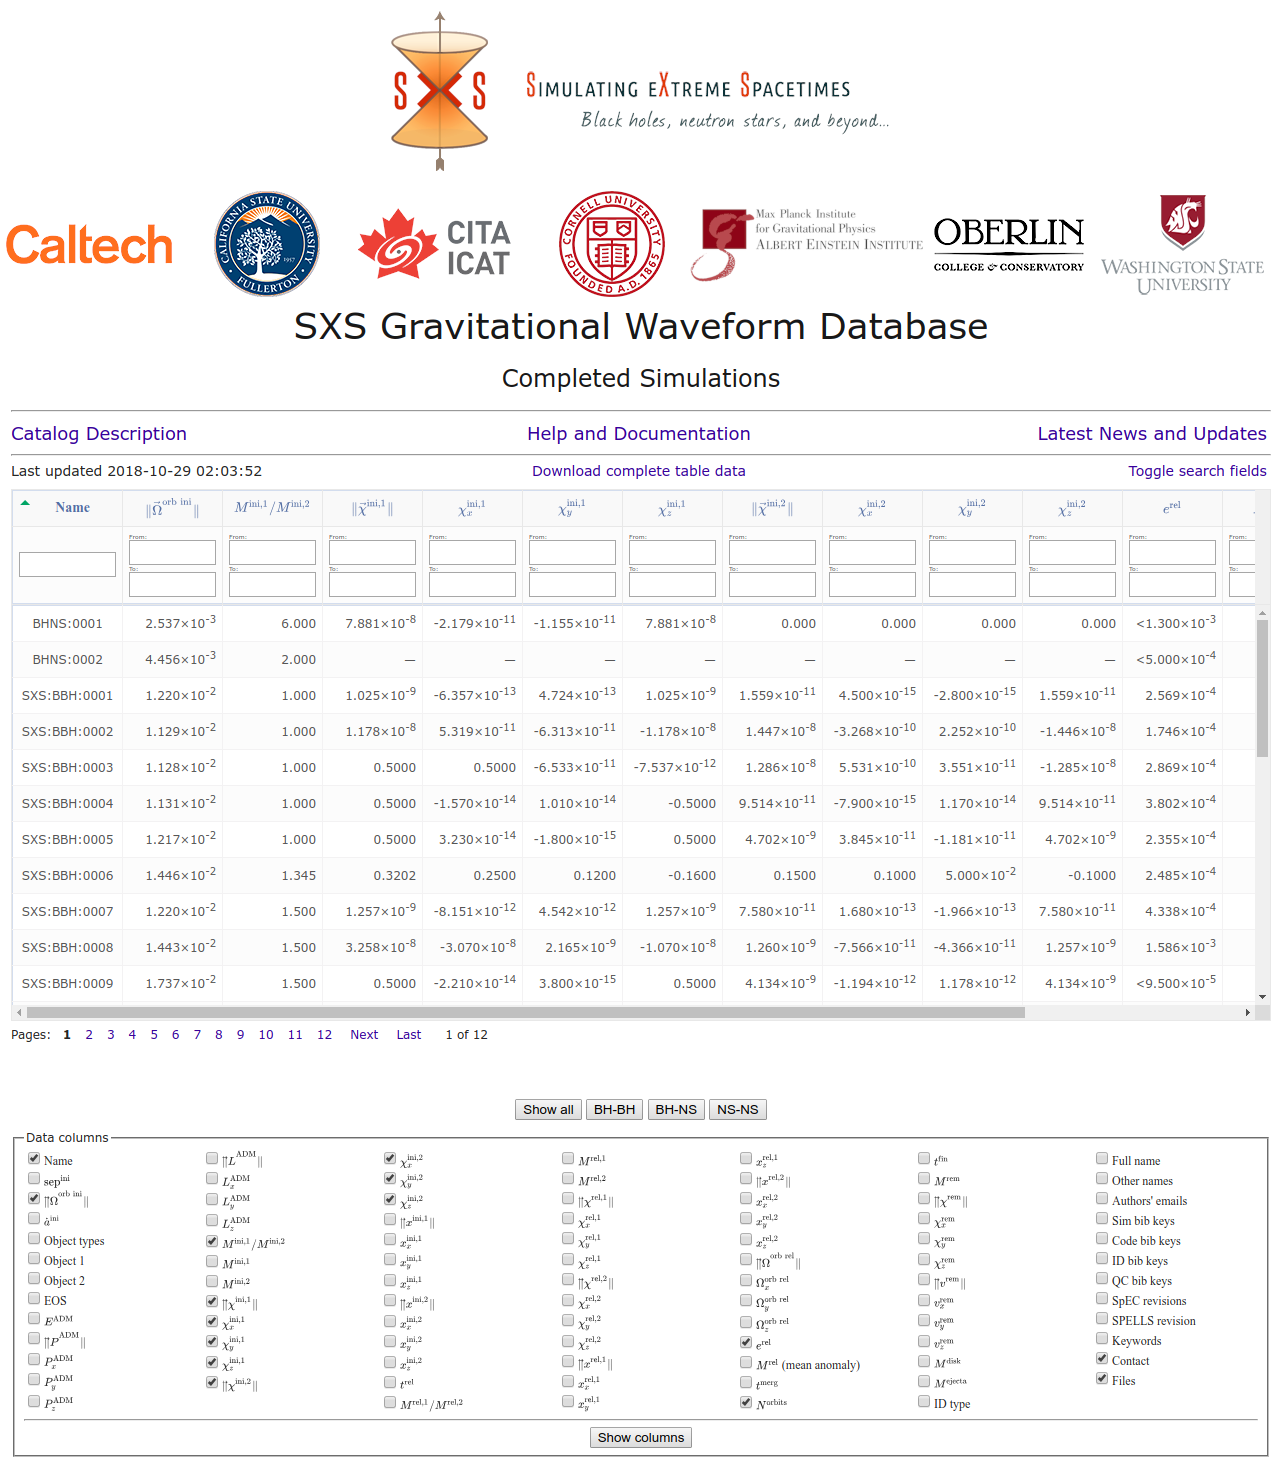
\includegraphics[width=1\textwidth]{figuras/sxs.png}
\caption{Banco de dados de de ondas gravitacionais SXS \href{https://www.black-holes.org/waveforms/catalog.php}{https://www.black-holes.org/waveforms/catalog.php} complementado com as instituições participantes e organizações de financiamento [SXS].}
\label{figsxs}
\end{figure}

A partir desta colaboração entre varias instituições e pesquisadores em 13 de outubro de 2013 um catalogo de simulações de ondas gravitacionais compreendendo 174 formas de onda e que atualmente existem 1377 simulações disponíveis que podem ser baixadas via wget\footnote{\href{https://www.gnu.org/software/wget/}{https://www.gnu.org/software/wget/ (02.12.2018)}} ou diretamente no navegador da web que conta com um litros restringindo os parâmetros (relação de massa, spins, excentricidade, órbitas etc.).

De acordo com a documentação do catalogo as ondas gravitacionais são descartáveis em várias resoluções (variando com o número de simulação individual) e diferentes ordens de extrapolação. Os rótulos de resolução Lev1, Lev2, ... são apenas uma quantidade relativa em uma simulação individual e não são comparáveis entre simulações com parâmetros diferentes. 

A precisão numérica depende da resolução, enquanto a precisão da extrapolação pode ser avaliada pela comparação de diferentes ordens de extrapolação. Pedidos mais altos tendem a produzir melhores resultados no inspiral, mas pior na parte de ringdown \cite{philipp}. 

Desta forma optará por buscar os rótulos de níveis mais elevados nas simulações devido a resultados mais atualizados e mais precisos. Para a facilidade em adquirir os dados será usado um algoritmo automatizado para baixar as simulações via wget, desenvolvido em Python\footnote{\href{https://www.python.org/}{https://www.python.org/ (02.12.2018)}}.

\section{Análise de Dados}
A primeira etapa do processo foi definir quais dados eram importantes e quais poderiam ser utilizados para se obter bons resultados na RNA.

A escolha e adequação dos dados utilizados para treinar e testar uma RNA é de fundamental importância. É necessário que se disponha de dados em quantidade e qualidade suficientes. Caso a quantidade de dados seja pequena, a rede não conseguirá criar um modelo suficientemente representativo para se ter um desempenho satisfatório quando aplicado em situações reais após o seu desenvolvimento, o que é chamado de sobre-ajuste (overfitting) dos dados. Além disto, os dados devem englobar todos os aspectos do problema em questão, a fim de que o modelo
criado seja genérico. Em geral, tais dados precisam ser convertidos para um formato padrão para utilização pelas RNAs. 

Com o objetivo de treinar uma RNA que forneça um diagnóstico classificativo das ondas gravitacionais e que apresente um bom desempenho, os dados colhidos serão tratados, conforme comentado a seguir. 

A descrição do catalogo afirma que dentro de cada simulação tem uma determinada ordem de extrapolação e resolução, a forma de onda é decomposta em harmônicos esféricos ponderados por spin-2 de índices multipolares L de 2 a 8 e M entre +L e −L incluindo 0. Existem imensas diferenças até um fator de \(10^{−7}\) entre determinados modos e o modo dominante (L, M) = (2, 2). Se o fator exceder \(10^{-5}\), os mantenedores do catálogo de ondas gravitacionais recomendam não confiar na precisão do modo específico, porque podem ser tão pequenos que são um ruído puramente numérico.

Portanto, os dados devem ser passados por um tratamento retirando as informações imprecisas das simulações, de modo que, reste somente as informações uteis.

Decerto não será possível usar de todas as simulações advindas do catalogo SXS, dessa forma, inicialmente deverá ser usado somente um grupo de dados destas simulações, para que isto seja possível, ocorrerá o desenvolvimento de um algoritmo que agrupe as simulações com características de spin semelhantes e relação de massas diferentes, a Figura~\ref{figclusterizacao} ilustra como uma porção das simulações esta distribuídas.

\begin{figure}[ht]
\centering
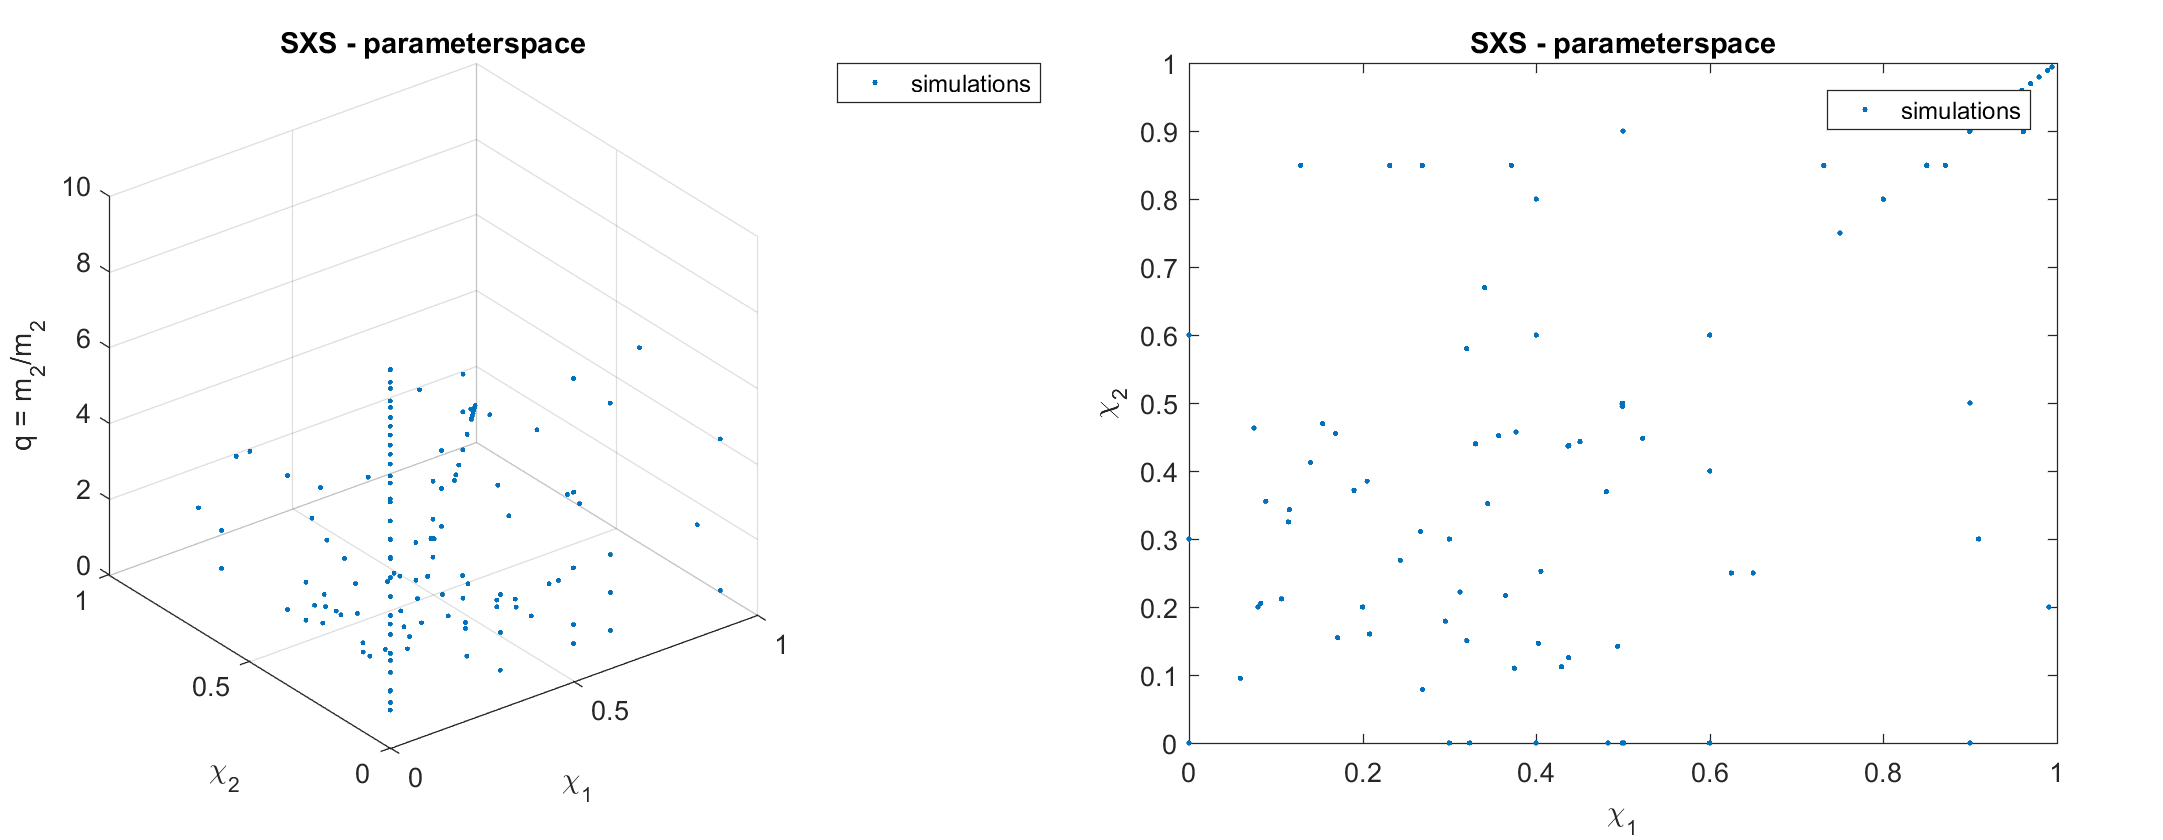
\includegraphics[width=1\textwidth]{figuras/clusterizacao.png}
\caption{Parâmetros do SXS: Dados iniciais em 3D (esquerda) incluindo a taxa de massa \({\nu}\) e 2D (direita) com apenas os spins individuais \(X_1\) e \(X_2\). [Image: \citeonline{philipp}.}
\label{figclusterizacao}
\end{figure}

Em seguida, precisará ser feita a escolha do grupo de simulações com maior quantidade de simulações. em cada simulação existe cerca de 8 arquivos (excluindo os metadados), 6 destes contêm dados de ondas gravitacionais, enquanto 2 descrevem a evolução das órbitas, rotações e outras grandezas geométricas, como a curvatura do espaço-tempo junto com o campo de maré e arrastamento de quadro no Buraco Negro. Com exceção do metadata.txt, os arquivos estão no Formato de Dados Hierárquicos (HDF5) [HDF] com a extensão de arquivo .h5.

Como descrito pelo catalogo, existe comumente dois arquivos com ondas gravitações de maior precisão, são eles,
\textbf{rh\_FiniteRadii\_CodeUnits.h5} e \\
\textbf{rPsi4\_FiniteRadii\_CodeUnits.h5}, esses dois arquivos contêm saída bruta de simulações nas quais as quantidades h e \(\Psi_{4}\) são extraídas em vários raios finitos com grupos h5 rotulados como "Rxxxx.dir", onde "xxxx" é o raio coordenado arredondado para o inteiro mais próximo.

Nas palavras de \cite{philipp}, o arquivo \textbf{rPsi4\_FiniteRadii\_CodeUnits.h5} é o que contem a melhor precisão, dado que representa o melhor estado da arte. Por este motivo o arquivo será usado nesta pesquisa, dentro dele existe varias observações com diferentes esféricos harmônicos, incluindo mais quatro dados que não serão usados nesta pesquisa, por este motivo na analise do arquivo, a Figura~\ref{figpsi4} ilustra o arquivo \textbf{rPsi4\_FiniteRadii\_CodeUnits.h5} aberto em um programa de visualização HDF.

\begin{figure}[ht]
\centering
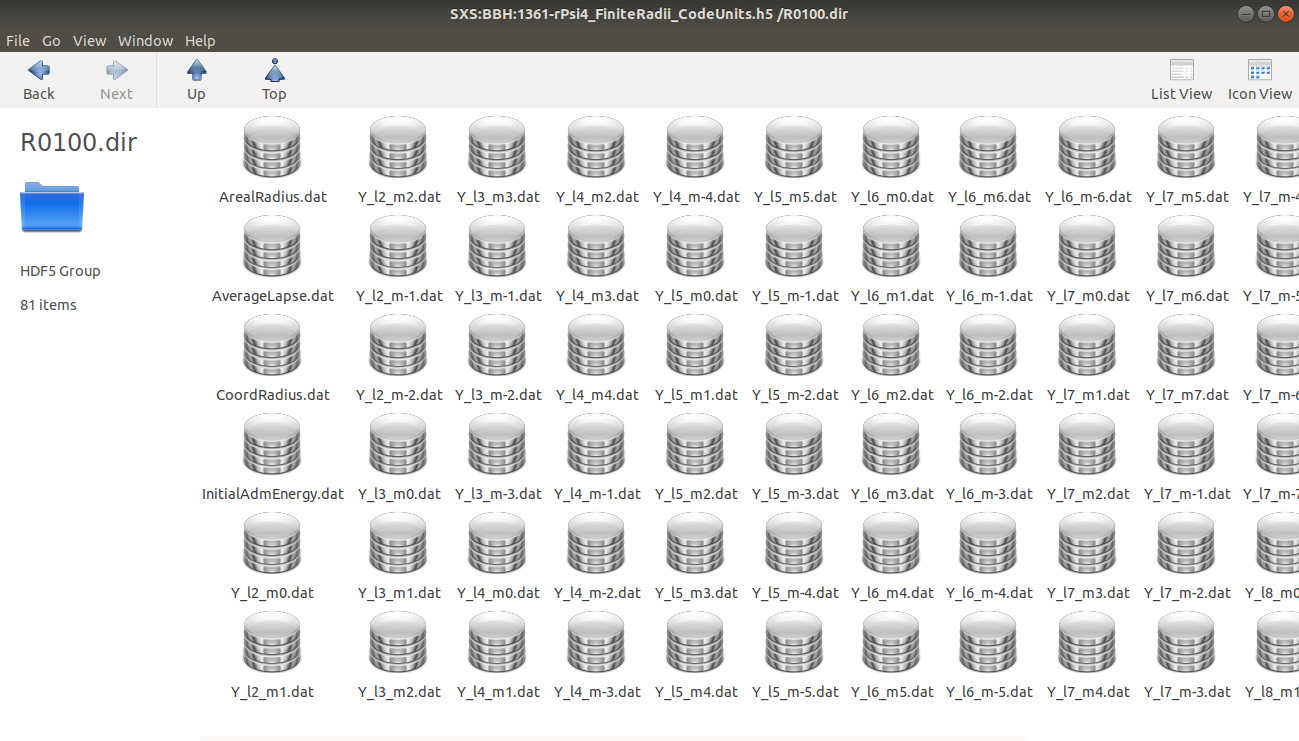
\includegraphics[width=1\textwidth]{figuras/arquivorhpsi4.png}
\caption{Arquivo \textbf{rPsi4\_FiniteRadii\_CodeUnits.h5} aberto com o programa HDFCompass.}
\label{figpsi4}
\end{figure}

Como mencionado anteriormente os harmônicos esféricos ponderados multipolares L e M, quando muito diferentes um do outro podem gerar dados imprecisos, diante disto, necessitará de uma limpeza nos dados a fim de sobrar somente aqueles com os dados que caracterizem  melhor as ondas gravitacionais.

\section{Desenho da pesquisa}
Para a conclusão dos objetivos propostos nesta pesquisa serão realizados algumas etapas as quais visão delinear este trabalho de forma sistemática a fim de garantir o direcionamento da mesma. 

A realização da pesquisa deste trabalho será embasada em experimentos, simulações e análises de dados, seguindo o fluxograma ilustrado na Figura~\ref{figpesquisa}. De forma mais direta, inicialmente a pesquisa constituirá de uma filtragem simplificada dos dados obtidos do grupo SXS, através de técnicas de series temporais afim de trata-los e padronizar os dados para os experimentos. Existem diversas formas de analisar e filtrar dados de series temporais, mais comumente utilizadas como por exemplo os modelos:

\begin{figure}[ht]
\centering
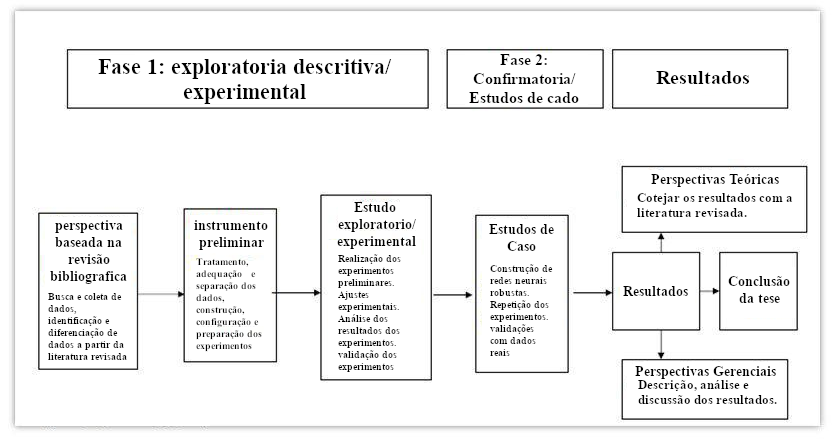
\includegraphics[width=1\textwidth]{figuras/desenho_da_pesquisa.png}
\caption{Desenho da pesquisa}
\label{figpesquisa}
\end{figure}

1 AR(p) → Modelo Auto-Regressivo de Ordem p;

2 MA(q) → Modelo Médias Móveis de Ordem q;

3 ARMA(p, q) → Modelo que combina AR(p) e MA(p);

4 ARIMA(p, d, q) → Modelo ARMA(p, q) com diferenciação de Ordem d.

Sendo que, em primeiro momento, não existirá a necessidade de se utilizar alguma dessas técnicas de analises avançadas, em principio será utilizada somente uma normalização dos dados e uma previa separação de 3 níveis, em que, todas serão padronizadas com a retirada da sua derivada e somadas a uma variação de ruídos uniformes e galicanos que variam entre 10\% e 100\%.

Os níveis gerados após este tratamento de dados serão diferenciados pela janela de informação contida em cada um dos níveis, sendo que, cada um terá um decimo de informação do nível anterior, ilustrado na Figura~\ref{figjanela}, começando com o nível um, o qual, não tem nível anterior e portanto terá uma janela de dados de 8192 pontos, seguido do segundo nível, em que, tem uma janela de informação de 819 pontos e por ultimo o terceiro nível que tem 82 pontos. As janelas de dados possuirão 10\% de sobreposição uma das outras, assim como mostra a Figura~\ref{figjanela}.

\begin{figure}[ht]
\centering
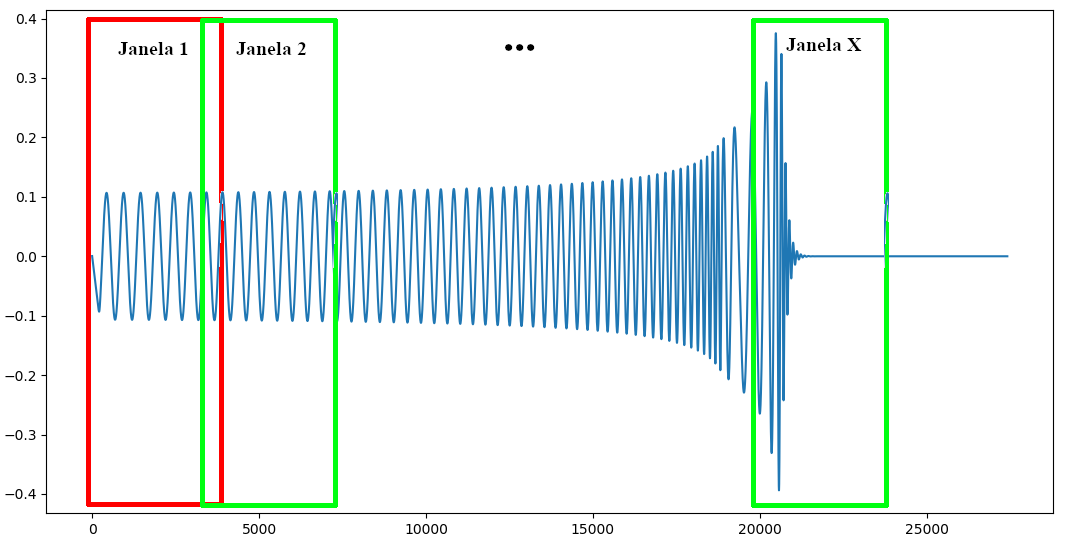
\includegraphics[width=1\textwidth]{figuras/janelas.png}
\caption{Janelas de informação com sobreposição}
\label{figjanela}
\end{figure}

Para obter os resultados e respostas acerca da problematização apresentada neste trabalho, será montado um experimento com redes neurais artificiais do tipo perceptron, mais especificamente do tipo MultiLayerPerceptron, sendo o treinamento realizado através do metodo backpropagation, baseado no método de experimentação dos quadrados latinos, sem a necessidade da analise estatística, conforme é demostrado na Figura~\ref{figexperimento}. No experimento será feita a análise sobre a separabilidade do sinal de informação das ondas gravitacionais e o ruido atrelado a ele, será usado o teste Kolmogorov–Smirnov (também conhecido como teste KS ou teste K–S), o qual, será medido a distancia KS de cada um dos resultados do experimento, ilustrado na Figura~\ref{figkolmogorov}, afim de descobrir o nível de separação das ondas gravitacionais do ruido.

\begin{figure}[ht]
\centering
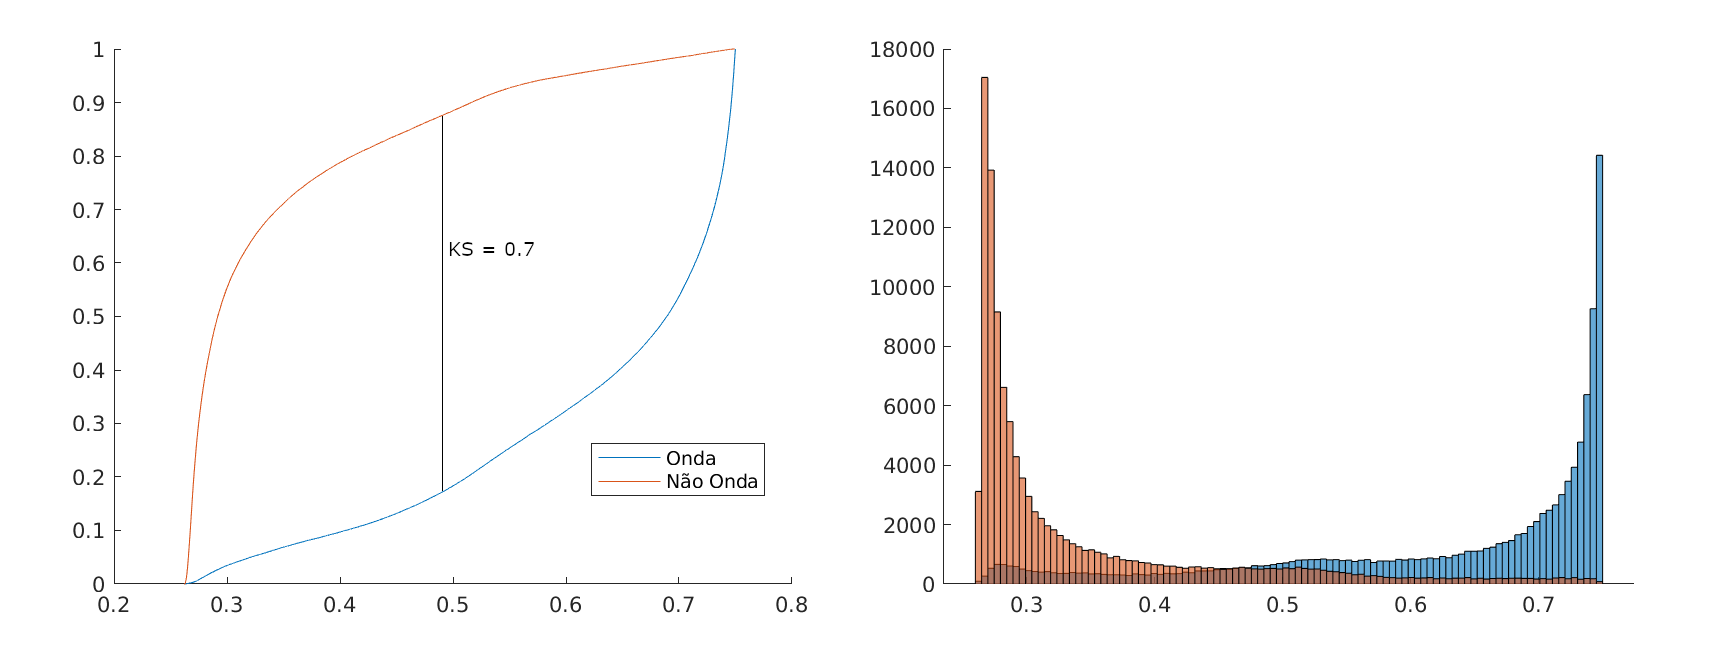
\includegraphics[width=1\textwidth]{figuras/test-kolmogorov.png}
\caption{Gráfico com exemplo do calculo da distancia KS (esquerda) e um Histograma demostrando a separabilidade de classificação.}
\label{figkolmogorov}
\end{figure}

\begin{figure}[ht]
\centering
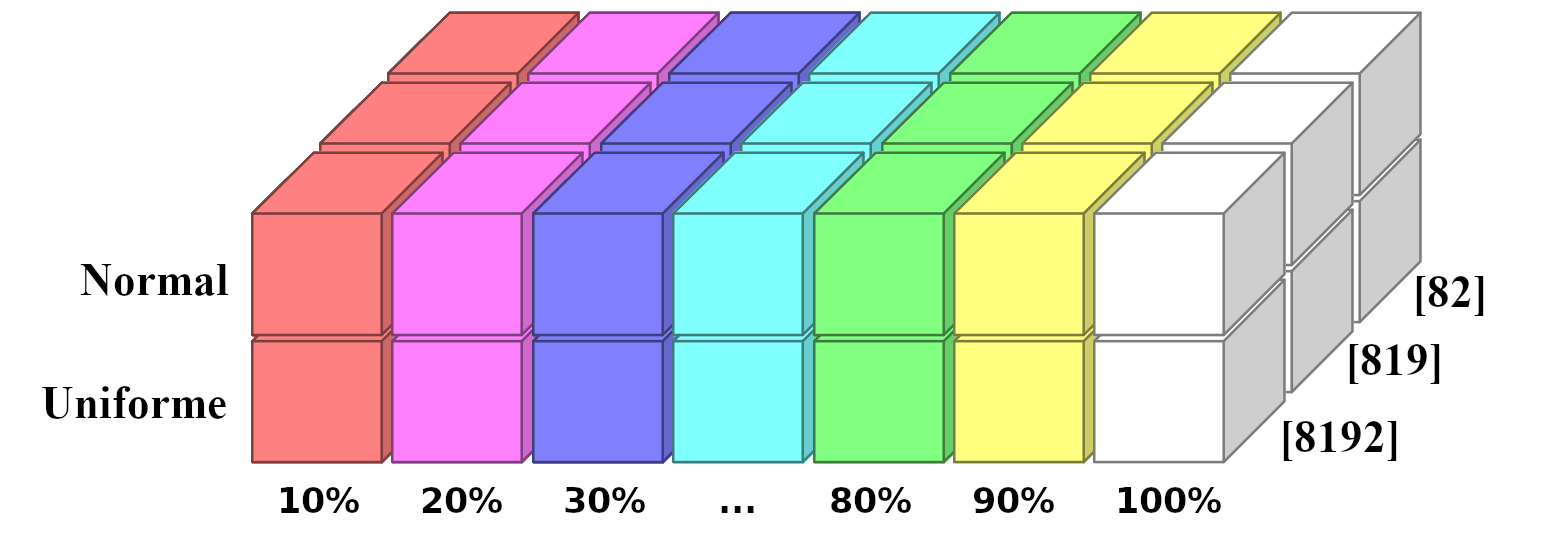
\includegraphics[width=1\textwidth]{figuras/experimento.png}
\caption{Experimento proposto}
\label{figexperimento}
\end{figure}

A rede neural artificial que será usada terá somente duas camadas, sendo, uma de entrada e uma de saída, que contaram com 10 neurônios na primeira camada e 2 neurônios na segunda camada, conforme ilustrado na Figura XX. Como os dados foram separados em 3 níveis, em que, cada um tem uma janela de informações diferente, cada experimento se adequará a este tipo de janela, sendo assim, a rede neural artificial terá uma quantidade de entrada(input) diferente para cada experimento, o qual, mudará o nível da janela de informação.

Após os resultados do primeiro experimento, sucederá uma nova etapa na pesquisa cujo delineamento dar-se-á para testes computacionais com diferentes abordagens de redes neurais artificiais, sendo elas, extreme learnign, Deep e Convulational. seguindo a mesma metodologia da primeira etapa desta pesquisa, desenrolar-se-á, os experimentos feitos anteriormente com abordagens de redes neurais artificiais diferentes para cada experimento, também calculando a distancia de Kolmogorov-Smirnov.

Logo depois de todos os experimentos serem feitos, haverá a necessidade de se fazer uma validação dos experimentos com os dados reais extraídos do LIGO, os quais, serão usados para validação dos experimentos e classificação dos resultados obtidos pelos mesmos.

E finalmente entraremos na etapa final, a qual, será para as analises dos resultados. Nesta analise haverá a necessidade de  se extrair todas as informações possíveis para se alcançar os objetivos desta pesquisa, para começar deverá ser feita uma categorização de todos os KS obtidos através dos experimentos para então classificar a melhor rede e ao mesmo tempo determinar que tipo de ruido existe nos dados reais e em qual amplitude os compõem.

Os resultados obtidos pela analise final serão cotejados com os resultados da literatura revisada. Dado que se os resultados forem satisfatórios, sucederá a descrição, analise e discussão dos resultados, afim de finalizar com a conclusão da escrita da dissertação e a submissão de artigos para revistas e eventos, concluindo assim o mestrado.